% =====================================================================
% Rapport final - Evaluation comparative de solutions de securite
% Compilation : pdflatex rapport_final.tex (deux fois pour la table des matieres)
% Les images sont lues dans ../../results/ et ../../docs/captures/ (depot Git)
% Sur Overleaf : envoyer ce fichier + les dossiers results/ et captures/ a cote
% =====================================================================
\documentclass[11pt,a4paper]{article}

\usepackage[utf8]{inputenc}
\usepackage[T1]{fontenc}
\usepackage{lmodern}
\usepackage[french]{babel}
\usepackage[a4paper,margin=2.4cm]{geometry}
\usepackage{graphicx}
\usepackage{booktabs}
\usepackage{tabularx}
\usepackage{array}
\usepackage{multirow}
\usepackage{caption}
\usepackage{subcaption}
\usepackage{float}
\usepackage{xcolor}
\usepackage{listings}
\usepackage{enumitem}
\usepackage{amssymb}
\usepackage{microtype}
\usepackage[colorlinks=true,linkcolor=blue!50!black,urlcolor=blue!50!black]{hyperref}

\graphicspath{{../../results/}{../../docs/captures/}{results/}{captures/}}

\setlist{itemsep=2pt,topsep=4pt}
\setlength{\parindent}{0pt}
\setlength{\parskip}{5pt}
\renewcommand{\arraystretch}{1.15}
\captionsetup{font=small,labelfont=bf}

\lstset{
  basicstyle=\ttfamily\footnotesize,
  backgroundcolor=\color{black!4},
  frame=single, rulecolor=\color{black!20},
  breaklines=true, columns=fullflexible,
  xleftmargin=4pt, xrightmargin=4pt
}

% Noms des auteurs : a adapter
\newcommand{\auteurA}{Nessryne Chouchene}
\newcommand{\auteurB}{Oumayma (B)}

\newcommand{\fic}[1]{\texttt{#1}}
\newcolumntype{Y}{>{\raggedright\arraybackslash}X}

\title{\textbf{Évaluation comparative de solutions de sécurité}\\[4pt]
\large Algorithmes, hachage de mots de passe, protocoles réseau, IDS et pare-feu}
\author{A : \auteurA\ (cryptographie, mots de passe)\\
B : \auteurB\ (protocoles, IDS et pare-feu)}
\date{Mini-projet sécurité -- rapport final}

\begin{document}
\maketitle
\thispagestyle{empty}
\tableofcontents
\newpage

% ---------------------------------------------------------------------
\section{Introduction et problématique}

Quelles solutions de sécurité (protocoles, algorithmes, hachage de mots de passe, système de
détection d'intrusion) faut-il choisir pour protéger une communication réseau, en fonction de la
sécurité apportée, des performances et de la complexité de configuration ?

Le projet ne consiste pas à utiliser des mécanismes de sécurité déjà prêts, mais à les
\emph{configurer, les attaquer, les mesurer et les comparer}, puis à recommander un choix
argumenté selon le besoin. Quatre comparaisons structurent le travail :
\begin{itemize}
  \item \textbf{C1} -- algorithmes cryptographiques (chiffrement, signature, hachage) ;
  \item \textbf{C2} -- hachage de mots de passe ;
  \item \textbf{C3} -- protocoles de protection du trafic réseau (TLS, WireGuard, tunnel SSH) ;
  \item \textbf{C4} -- système de détection d'intrusion (IDS, Suricata) et pare-feu (nftables).
\end{itemize}
Les comparaisons C1 et C2 ont été menées par A, les comparaisons C3 et C4 par B.
L'architecture, la méthode, la synthèse et la conclusion sont communes.

% ---------------------------------------------------------------------
\section{Architecture du laboratoire}

Le laboratoire repose sur un réseau virtuel interne (VirtualBox), isolé du reste du PC hôte
pendant les phases d'attaque. Une carte réseau NAT temporaire sert uniquement à installer les
paquets logiciels ; elle n'intervient dans aucune mesure ni aucune attaque.

\begin{table}[H]
\centering
\begin{tabularx}{\textwidth}{l l l c Y}
\toprule
\textbf{VM} & \textbf{Rôle} & \textbf{IP (réseau interne)} & \textbf{RAM} & \textbf{Fonctions} \\
\midrule
Client & Client / attaquant & 10.0.0.10 & 2 Go & Génère le trafic de référence, lance Nmap, Hydra, les mesures iperf3 et curl \\
Serveur & Serveur / défense & 10.0.0.20 & 2 Go & Héberge SSH, le serveur web, iperf3, les points d'entrée TLS, WireGuard et SSH, ainsi que l'IDS Suricata et le pare-feu nftables \\
\bottomrule
\end{tabularx}
\caption{Machines virtuelles du laboratoire (réseau interne \texttt{labnet}).}
\end{table}

Pour des raisons de ressources, l'IDS n'a pas été déployé sur une VM séparée mais directement
sur le Serveur, en écoute sur l'interface \texttt{enp0s8} (le réseau interne) -- option prévue
dès la conception du laboratoire.

Les deux VMs de la partie B tournent sous Lubuntu 24.04 LTS (noyau 7.0.0-43-generic), avec
2~vCPU chacune. L'interface graphique a été désactivée (\texttt{multi-user.target}) pendant les
phases de mesure, car l'économiseur d'écran par défaut consommait à lui seul environ 30~\% de
CPU sur chaque VM et faussait fortement les débits mesurés (un test a montré un débit
WireGuard de 44~Mbit/s avec l'interface graphique active contre 177~Mbit/s sans elle, toutes
choses égales par ailleurs).

Les mesures de la partie A (C1 et C2) ont été réalisées dans une VM client Lubuntu créée avec
Vagrant (base Ubuntu 22.04, 2~vCPU, 2~Go de RAM, John the Ripper 1.9.1 « jumbo »), décrite dans
\fic{vagrant/Vagrantfile}. Ces mesures sont purement locales (une seule machine) et ne
dépendent pas du réseau.

Captures associées : \fic{docs/captures/client\_ip.png}, \fic{serveur\_ip.png}, \fic{ping.png},
\fic{noyau.png}.

% ---------------------------------------------------------------------
\section{Méthode de comparaison}

\begin{itemize}
  \item \textbf{Critères fixés à l'avance} : sécurité (ce qu'un attaquant peut observer ou faire),
        performance (débit, latence, temps de calcul, charge CPU), complexité de configuration,
        cas d'usage conseillé.
  \item \textbf{Mêmes conditions de test} pour toutes les solutions comparées entre elles :
        mêmes VMs, interface graphique désactivée, aucune autre application active.
  \item \textbf{Répétitions} : 5 à 30 essais selon la mesure, moyenne retenue ; le premier essai
        d'une série de téléchargement est systématiquement exclu du calcul (effet de démarrage
        à froid observé).
  \item \textbf{Résultats enregistrés} en CSV dans \fic{results/}, un script ou une série de
        commandes par comparaison.
  \item \textbf{Preuve systématique} : une capture d'écran pour chaque configuration et chaque
        résultat d'attaque.
  \item \textbf{Éthique} : toutes les attaques (scan, brute force) sont réalisées exclusivement
        à l'intérieur du réseau virtuel isolé du projet, sur des machines et des comptes créés
        pour l'occasion.
\end{itemize}

\textbf{Limite méthodologique commune à C1--C4.} Les mesures absolues varient sensiblement
d'une session à l'autre dans l'environnement virtualisé (par exemple, le débit en clair mesuré
par iperf3 est passé de 791,8 à 864 puis 992~Mbit/s selon le jour, pour une configuration
strictement identique). Les comparaisons entre protocoles ne sont donc valables que lorsqu'elles
sont faites dans une même session de mesure, ce qui a été respecté pour tous les tableaux
comparatifs présentés ci-dessous. Les valeurs absolues isolées (une mesure unique, un seul jour)
sont à lire en ordre de grandeur plutôt qu'en valeur de référence universelle.

% ---------------------------------------------------------------------
\section{C1 -- Algorithmes cryptographiques (partie A)}

\subsection{Configuration}
Le script \fic{algorithms/bench\_c1.py} appelle \texttt{openssl speed} (blocs de 8~Ko) pour
AES-128 et AES-256 en modes CBC et GCM, SHA-256 et SHA3-256, puis RSA-2048, RSA-4096, ECDSA P-256
et Ed25519 (signatures et vérifications par seconde). Il génère aussi une clé par algorithme pour
relever la taille réelle des clés et des signatures. Chaque mesure est répétée 5 fois ; les valeurs
indiquées sont des moyennes.

\subsection{Résultats}

\begin{table}[H]
\centering
\begin{tabular}{l r}
\toprule
\textbf{Algorithme} & \textbf{Débit (Mo/s)} \\
\midrule
AES-128-GCM & 5\,432 \\
AES-256-GCM & 3\,484 \\
AES-128-CBC & 1\,652 \\
AES-256-CBC & 1\,117 \\
SHA-256 & 349 \\
SHA3-256 & 265 \\
\bottomrule
\end{tabular}
\caption{Débit symétrique et hachage (\fic{results/c1\_symetrique.csv}, moyennes sur 5 répétitions).}
\end{table}

\begin{table}[H]
\centering
\begin{tabular}{l r r}
\toprule
\textbf{Algorithme} & \textbf{Signatures/s} & \textbf{Vérifications/s} \\
\midrule
RSA-2048 & 1\,423 & 49\,019 \\
RSA-4096 & 293 & 19\,830 \\
ECDSA P-256 & 48\,967 & 18\,262 \\
Ed25519 & 26\,815 & 9\,994 \\
\bottomrule
\end{tabular}
\caption{Algorithmes asymétriques (\fic{results/c1\_asymetrique.csv}).}
\end{table}

\begin{table}[H]
\centering
\begin{tabular}{l r r r}
\toprule
\textbf{Algorithme} & \textbf{Clé publique (o)} & \textbf{Clé privée (o)} & \textbf{Signature (o)} \\
\midrule
RSA-2048 & 294 & 1\,191 & 256 \\
RSA-4096 & 550 & 2\,347 & 512 \\
ECDSA P-256 & 91 & 121 & 71 (DER) \\
Ed25519 & 44 & 48 & 64 \\
\bottomrule
\end{tabular}
\caption{Tailles réelles des clés et des signatures (\fic{results/c1\_tailles.csv}).}
\end{table}

\begin{figure}[H]
\centering
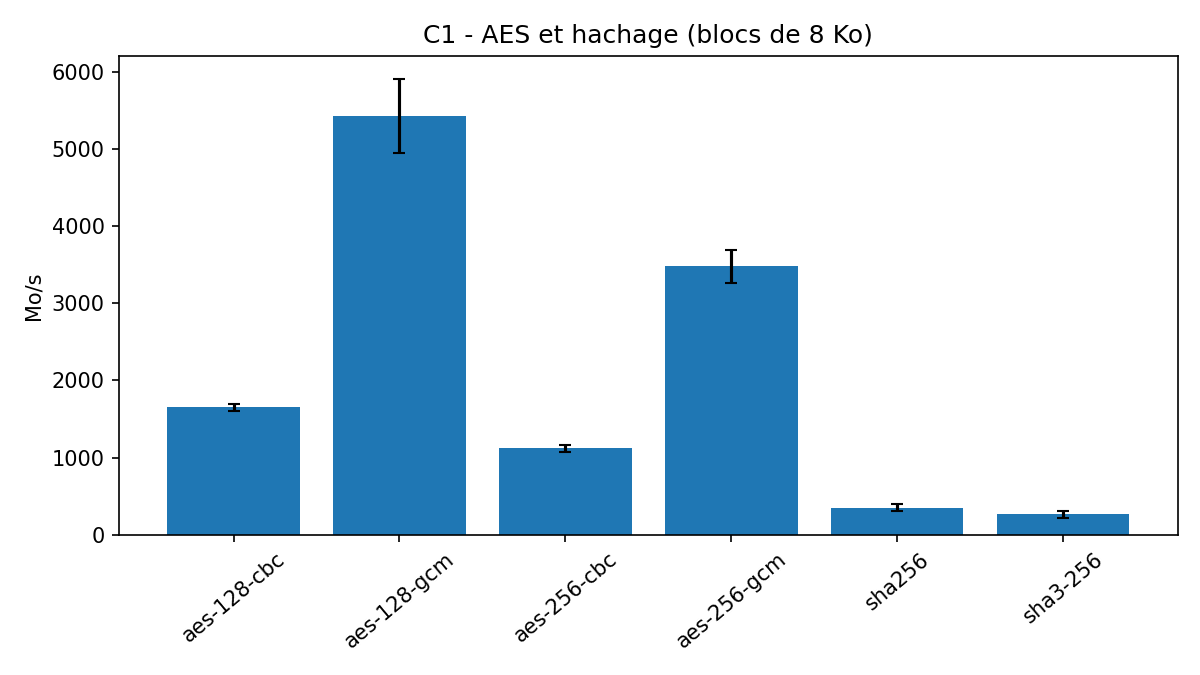
\includegraphics[width=0.48\textwidth]{c1_symetrique.png}\hfill
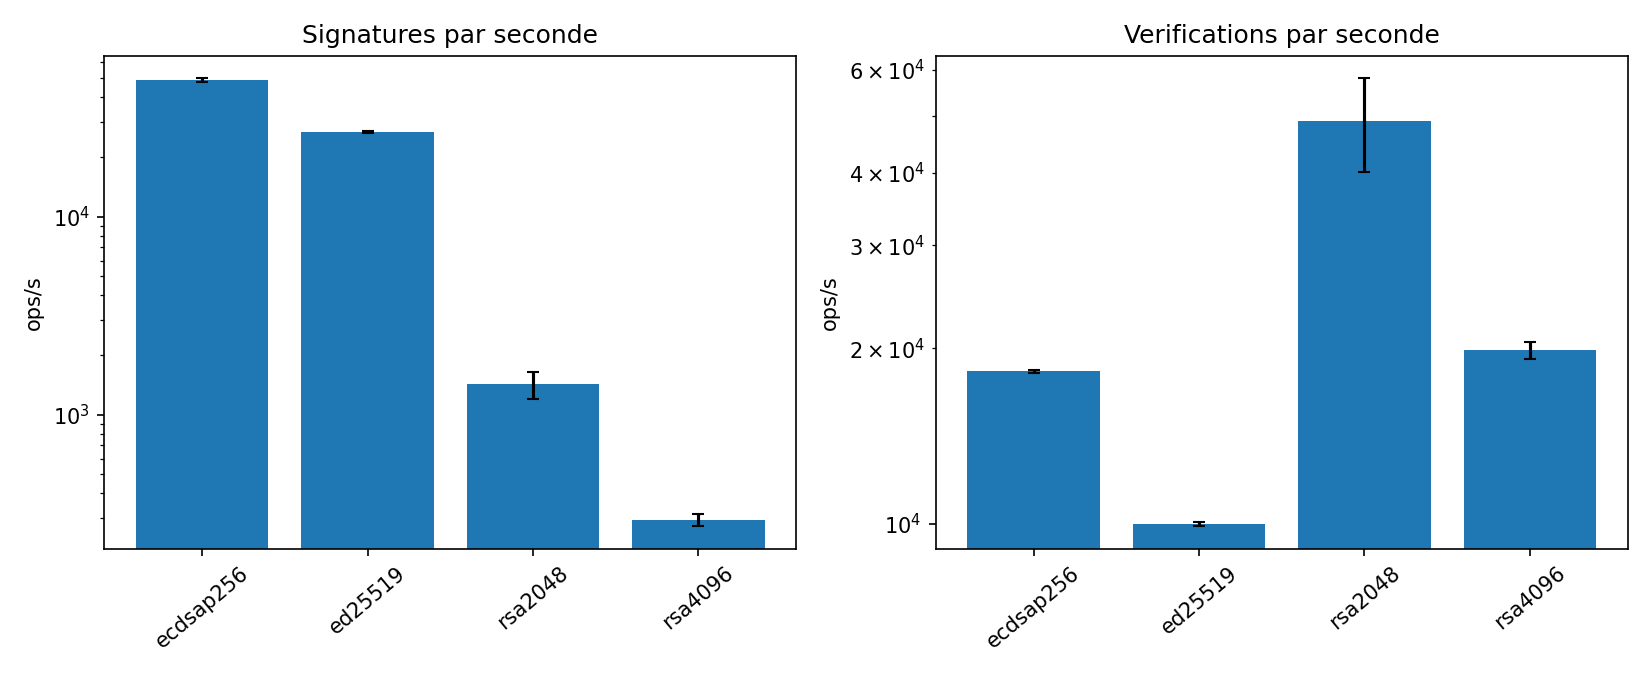
\includegraphics[width=0.48\textwidth]{c1_asymetrique.png}
\caption{C1 : débits symétriques (gauche) et opérations asymétriques par seconde (droite).}
\end{figure}

\subsection{Analyse}
\begin{itemize}
  \item \textbf{AES-GCM contre AES-CBC} : GCM fournit confidentialité \emph{et} intégrité
        (chiffrement authentifié) et se parallélise ; CBC ne fournit que la confidentialité,
        exige un MAC séparé et est exposé aux attaques de type \emph{padding oracle} s'il est
        mal utilisé. Mesuré : GCM est environ 3,3 fois plus rapide que CBC en AES-128
        (5\,432 contre 1\,652~Mo/s), car le chiffrement CBC est séquentiel.
  \item \textbf{AES-128 contre AES-256} : 256 bits coûte plus de calcul (14 tours contre 10) ;
        mesuré, AES-256-GCM est environ 36~\% plus lent qu'AES-128-GCM, pour un gain de sécurité
        jugé non nécessaire aujourd'hui (128 bits reste sûr).
  \item \textbf{RSA, ECDSA, Ed25519} : à niveau de sécurité comparable, les courbes elliptiques
        ont des clés et des signatures bien plus petites et une signature nettement plus rapide
        (48\,967 signatures/s pour ECDSA contre 1\,423 pour RSA-2048) ; RSA vérifie très vite mais
        signe lentement (surtout en 4096 bits). Ed25519 est déterministe, ce qui évite la
        fragilité d'ECDSA face à un nonce mal généré. RSA-2048 correspond à environ 112 bits de
        sécurité.
  \item \textbf{SHA-256 contre SHA3-256} : même taille de sortie, constructions différentes
        (Merkle--Damgård contre éponge). SHA-2 est plus rapide ici (349 contre 265~Mo/s) ;
        SHA-3 résiste nativement à l'extension de longueur.
\end{itemize}

% ---------------------------------------------------------------------
\section{C2 -- Hachage de mots de passe (partie A)}

\subsection{Configuration}
\begin{itemize}
  \item \fic{passwords/bench\_c2.py} mesure le temps de calcul par hash pour SHA-256 simple (sans
        sel), PBKDF2-HMAC-SHA256 (10\,000 / 100\,000 / 600\,000 itérations), bcrypt (coûts 8, 10,
        12, 14) et Argon2id (3 profils).
  \item \fic{passwords/gen\_data.py} génère une liste de candidats fixe (graine 42, 1\,000 mots)
        et 10 mots de passe de test (6 présents dans la liste, 4 absents), hachés avec chaque
        algorithme.
  \item \fic{passwords/crack\_c2.sh} lance John the Ripper sur CPU avec la même liste pour tous les
        algorithmes, 5 répétitions.
  \item Les coûts utilisés pour le craquage sont volontairement modestes (PBKDF2 = 10\,000
        itérations, bcrypt = coût 8, Argon2id = $t=1$, $m=8$~Mio, $p=1$), pour garder un temps de
        mesure raisonnable sur CPU.
\end{itemize}

\subsection{Résultats}

\begin{table}[H]
\centering
\begin{tabular}{l l r}
\toprule
\textbf{Algorithme} & \textbf{Paramètres} & \textbf{Temps par hash} \\
\midrule
SHA-256 simple & sans sel & 0,007 ms \\
\midrule
PBKDF2-HMAC-SHA256 & 10\,000 it. & 5,2 ms \\
 & 100\,000 it. & 49 ms \\
 & 600\,000 it. & 291 ms \\
\midrule
bcrypt & coût 8 & 13 ms \\
 & coût 10 & 51 ms \\
 & coût 12 & 203 ms \\
 & coût 14 & 827 ms \\
\midrule
Argon2id & $t=1$, 8 Mio & 7 ms \\
 & $t=2$, 19 Mio & 29 ms \\
 & $t=3$, 64 Mio & 185 ms \\
\bottomrule
\end{tabular}
\caption{Temps de calcul d'un hash (\fic{results/c2\_temps\_hash.csv}, moyenne sur 5 répétitions).}
\end{table}

\begin{table}[H]
\centering
\begin{tabular}{l r r r}
\toprule
\textbf{Algorithme (coût du test)} & \textbf{Trouvés} & \textbf{Temps moyen} & \textbf{ms/tentative} \\
\midrule
SHA-256 simple & 6/10 & 0,41 s & 0,04 \\
PBKDF2 (10\,000 it.) & 6/10 & 4,7 s & 0,47 \\
Argon2id ($t=1$, 8 Mio) & 6/10 & 10,2 s & 1,02 \\
bcrypt (coût 8) & 6/10 & 17,0 s & 1,69 \\
\bottomrule
\end{tabular}
\caption{Craquage avec John the Ripper (1\,000 candidats, 10 comptes, 5 répétitions ;
\fic{results/c2\_craquage.csv}). Une « tentative » est un mot de la liste essayé contre un compte.}
\end{table}

Avec ces coûts modestes, SHA-256 simple se casse environ 40 fois plus vite que bcrypt ; avec les
coûts recommandés en production (PBKDF2 600\,000 itérations, bcrypt 12, Argon2id 19~Mio),
l'écart serait bien plus grand.

\begin{figure}[H]
\centering
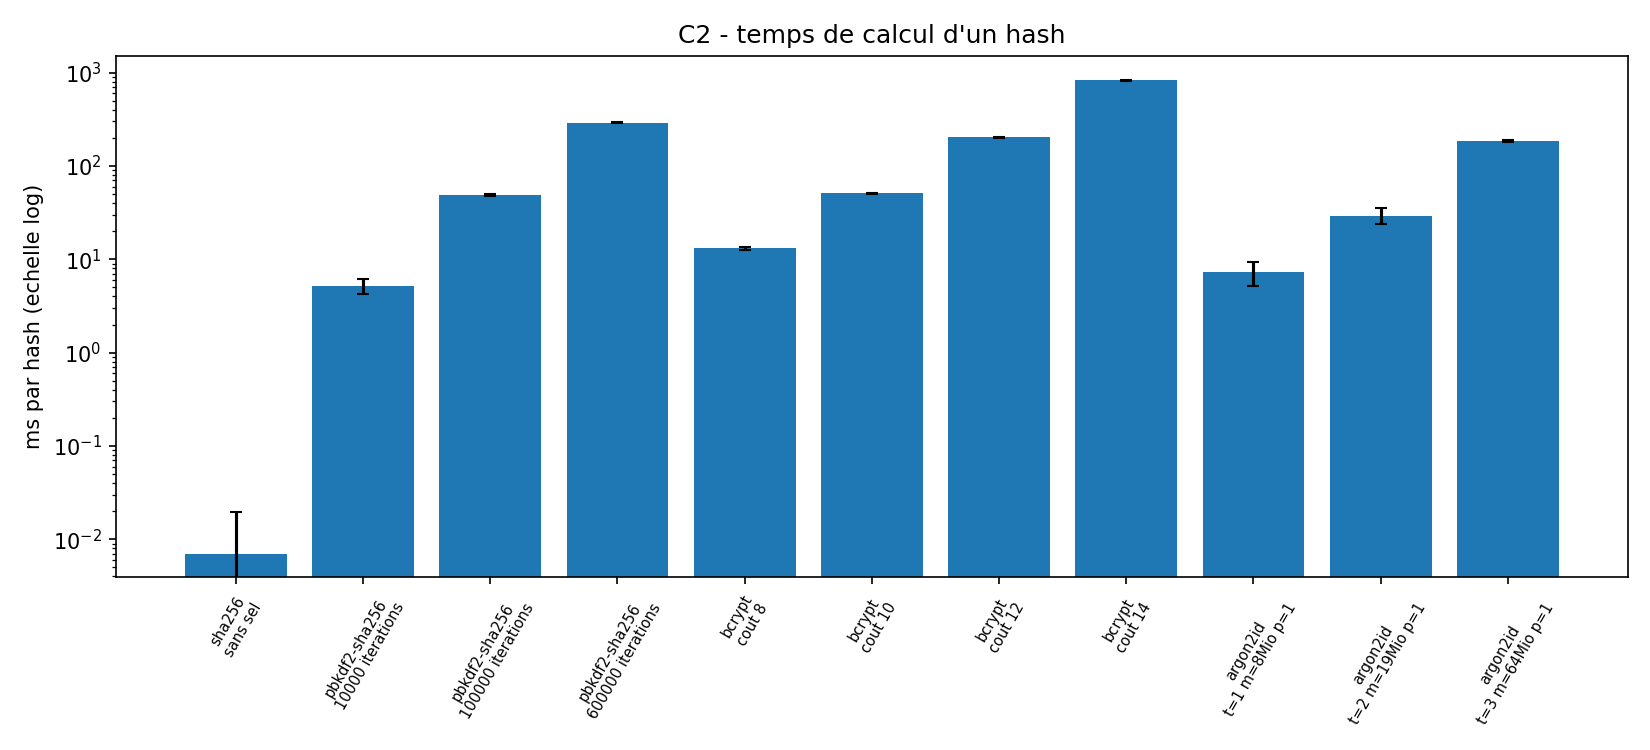
\includegraphics[width=0.52\textwidth]{c2_temps_hash.png}\hfill
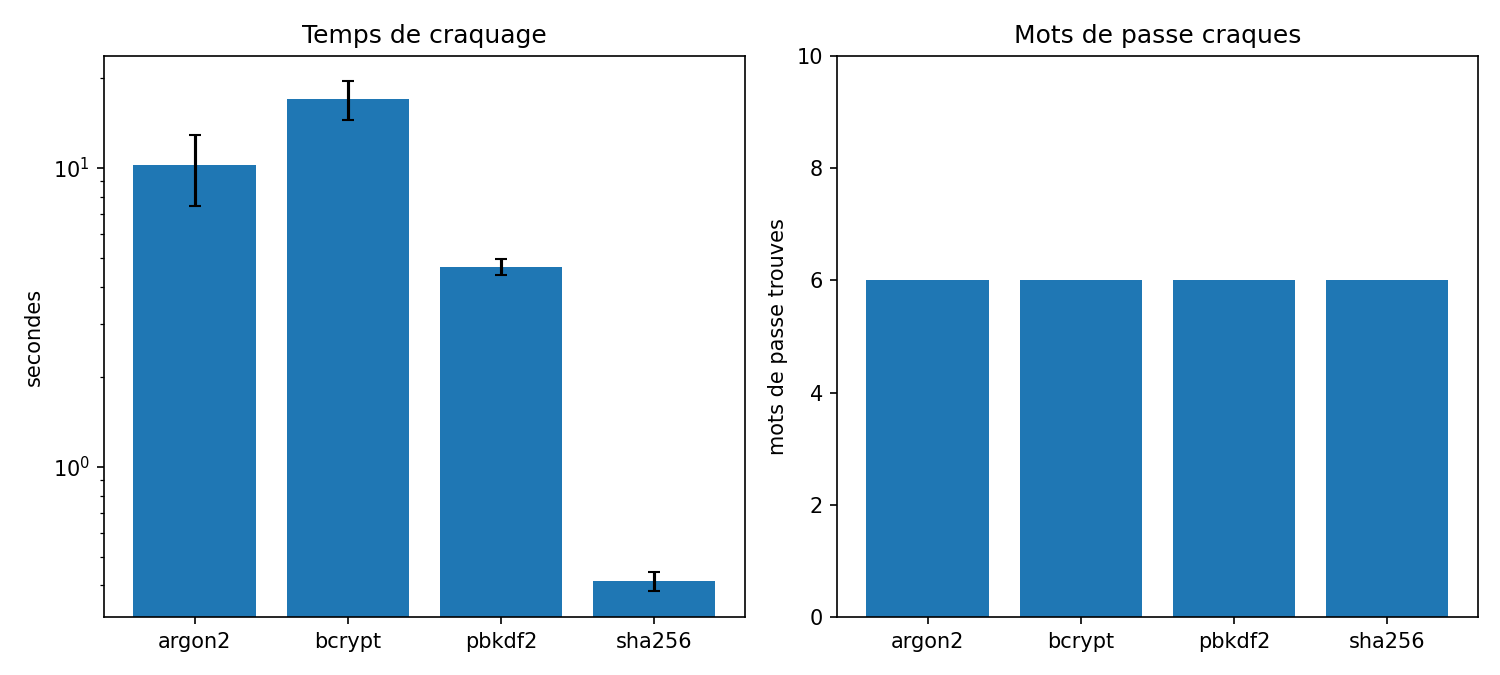
\includegraphics[width=0.44\textwidth]{c2_craquage.png}
\caption{C2 : temps de calcul d'un hash (échelle logarithmique) et résultats du craquage.}
\end{figure}

\subsection{Analyse}
\begin{itemize}
  \item Un hash rapide et non salé (SHA-256 simple) est inadapté aux mots de passe : un attaquant
        teste des millions de candidats par seconde, et deux utilisateurs au même mot de passe
        produisent le même hash.
  \item Les trois autres algorithmes sont lents, salés et à coût réglable. Recommandations OWASP :
        Argon2id ($m \geq 19$~Mio, $t \geq 2$, $p = 1$) en premier choix, sinon bcrypt (coût
        $\geq 10$) ou PBKDF2-HMAC-SHA256 ($\geq 600\,000$ itérations).
  \item Argon2id est \emph{memory-hard} et résiste mieux au matériel parallèle (GPU, ASIC). bcrypt
        est éprouvé mais ignore les octets d'un mot de passe au-delà de 72. PBKDF2 est
        standardisé (FIPS) mais moins résistant au matériel parallèle.
  \item \textbf{Limite} : le craquage ne porte que sur des mots de passe présents dans le
        dictionnaire de test ; un mot de passe absent de la liste n'est retrouvé par aucun
        algorithme, ce qui souligne le rôle de la robustesse du mot de passe choisi par
        l'utilisateur, indépendamment de l'algorithme de hachage.
\end{itemize}

% ---------------------------------------------------------------------
\section{C3 -- Protocoles de protection du trafic (partie B)}

\subsection{Configurations testées}
Quatre situations ont été comparées pour un même échange Client $\rightarrow$ Serveur (une requête
HTTP contenant \texttt{mot\_de\_passe=secret123}, puis un fichier de 100~Mo) :

\begin{table}[H]
\centering
\begin{tabularx}{\textwidth}{l Y Y}
\toprule
\textbf{Configuration} & \textbf{Description} & \textbf{Fichier de configuration} \\
\midrule
Clair & Référence : serveur HTTP Python, aucune protection & -- \\
TLS & stunnel devant le serveur web, certificat auto-signé RSA-2048, TLS 1.3 & \fic{config/stunnel.conf} \\
WireGuard & Tunnel réseau complet (couche IP) entre les deux VMs, réseau 10.10.0.0/24 & \fic{config/wg0\_client.conf}, \fic{config/wg0\_serveur.conf} (sans clé privée) \\
SSH (tunnel) & Redirection de port (\texttt{ssh -L}) vers le serveur web, authentification par clé Ed25519 & -- (clé privée jamais commitée) \\
\bottomrule
\end{tabularx}
\caption{Configurations de protection comparées.}
\end{table}

IPsec (prévu initialement) a été remplacé par un tunnel SSH, après concertation, pour rester dans
le délai imparti tout en conservant un troisième point de comparaison pertinent (authentification
par clé plutôt que par certificat ou par échange de clés WireGuard).

TLS négocie automatiquement TLS 1.3, suite \texttt{TLS\_AES\_256\_GCM\_SHA384}, échange de clé X25519,
signature du serveur RSASSA-PSS. WireGuard utilise par construction ChaCha20-Poly1305, Curve25519
et BLAKE2s, sans négociation. SSH négocie par défaut un échange de clé hybride post-quantique
\texttt{sntrup761x25519-sha512@openssh.com}, une clé d'hôte Ed25519 et un chiffrement
ChaCha20-Poly1305 (OpenSSH 9.6).

\subsection{Mesures de performance (même session, interface graphique désactivée)}

\begin{table}[H]
\centering
\begin{tabularx}{\textwidth}{Y r r r r}
\toprule
\textbf{Mesure} & \textbf{Clair} & \textbf{TLS} & \textbf{WireGuard} & \textbf{SSH (tunnel)} \\
\midrule
Latence (ping, 50 paquets) & 2,08 ms & n/a* & 5,66 ms (+3,58) & n/a* \\
Petite requête (30 essais) & 7,87 ms & 22,56 ms (+14,69) & 12,48 ms (+4,61) & 19,29 ms (+11,42) \\
Poignée de main / ouverture & -- & 13,06 ms & -- & 493 ms (session SSH complète) \\
Débit, téléchargement 100 Mo (5 essais) & 613 Mbit/s & 459 Mbit/s (−25 \%) & 67 Mbit/s (−89 \%) & 400 Mbit/s (−35 \%) \\
\bottomrule
\end{tabularx}
\caption{Comparaison des protocoles. *Le ping utilise ICMP, qui n'est protégé ni par TLS
(limité à une connexion TCP applicative) ni par le tunnel SSH par redirection de port (limité au
trafic TCP redirigé) ; seul WireGuard, qui chiffre tout le trafic IP, protège aussi l'ICMP.}
\end{table}

Comparaison de deux chiffrements SSH (ChaCha20-Poly1305 contre AES-256-GCM, 5 essais alternés
chacun après exclusion du premier essai de chauffe) : 467~Mbit/s pour ChaCha20-Poly1305 contre
506~Mbit/s pour AES-256-GCM. Aucune différence significative n'a été observée (écart de 8~\%, dans
l'ordre de la variabilité habituelle des mesures), malgré la présence d'instructions matérielles
AES sur le processeur de la VM (\texttt{aes}, \texttt{avx2} détectés dans \texttt{/proc/cpuinfo}).

\subsection{Preuve de confidentialité (Wireshark)}
Pour chaque configuration, le même échange a été capturé sur l'interface \texttt{enp0s8} et analysé
dans Wireshark :

\begin{table}[H]
\centering
\begin{tabularx}{\textwidth}{l Y Y}
\toprule
\textbf{Configuration} & \textbf{Contenu de la requête} & \textbf{Recherche de \texttt{secret123} dans les octets} \\
\midrule
Clair & Lisible en texte brut (\texttt{mot\_de\_passe=secret123}) & Trouvé \\
TLS & Illisible (\emph{Application Data} chiffré) & Introuvable \\
WireGuard & Illisible (\emph{Transport Data} chiffré) & Introuvable \\
SSH & Illisible (\emph{Encrypted packet}) & Introuvable \\
\bottomrule
\end{tabularx}
\caption{Visibilité du mot de passe dans les captures.}
\end{table}

Dans les trois cas protégés, la négociation reste partiellement visible en clair (le Client Hello
TLS liste les suites de chiffrement proposées ; le Key Exchange Init SSH liste les algorithmes
proposés, y compris \texttt{sntrup761x25519-sha512}), mais jamais le contenu de la communication.

\begin{figure}[H]
\centering
\begin{subfigure}{0.48\textwidth}
  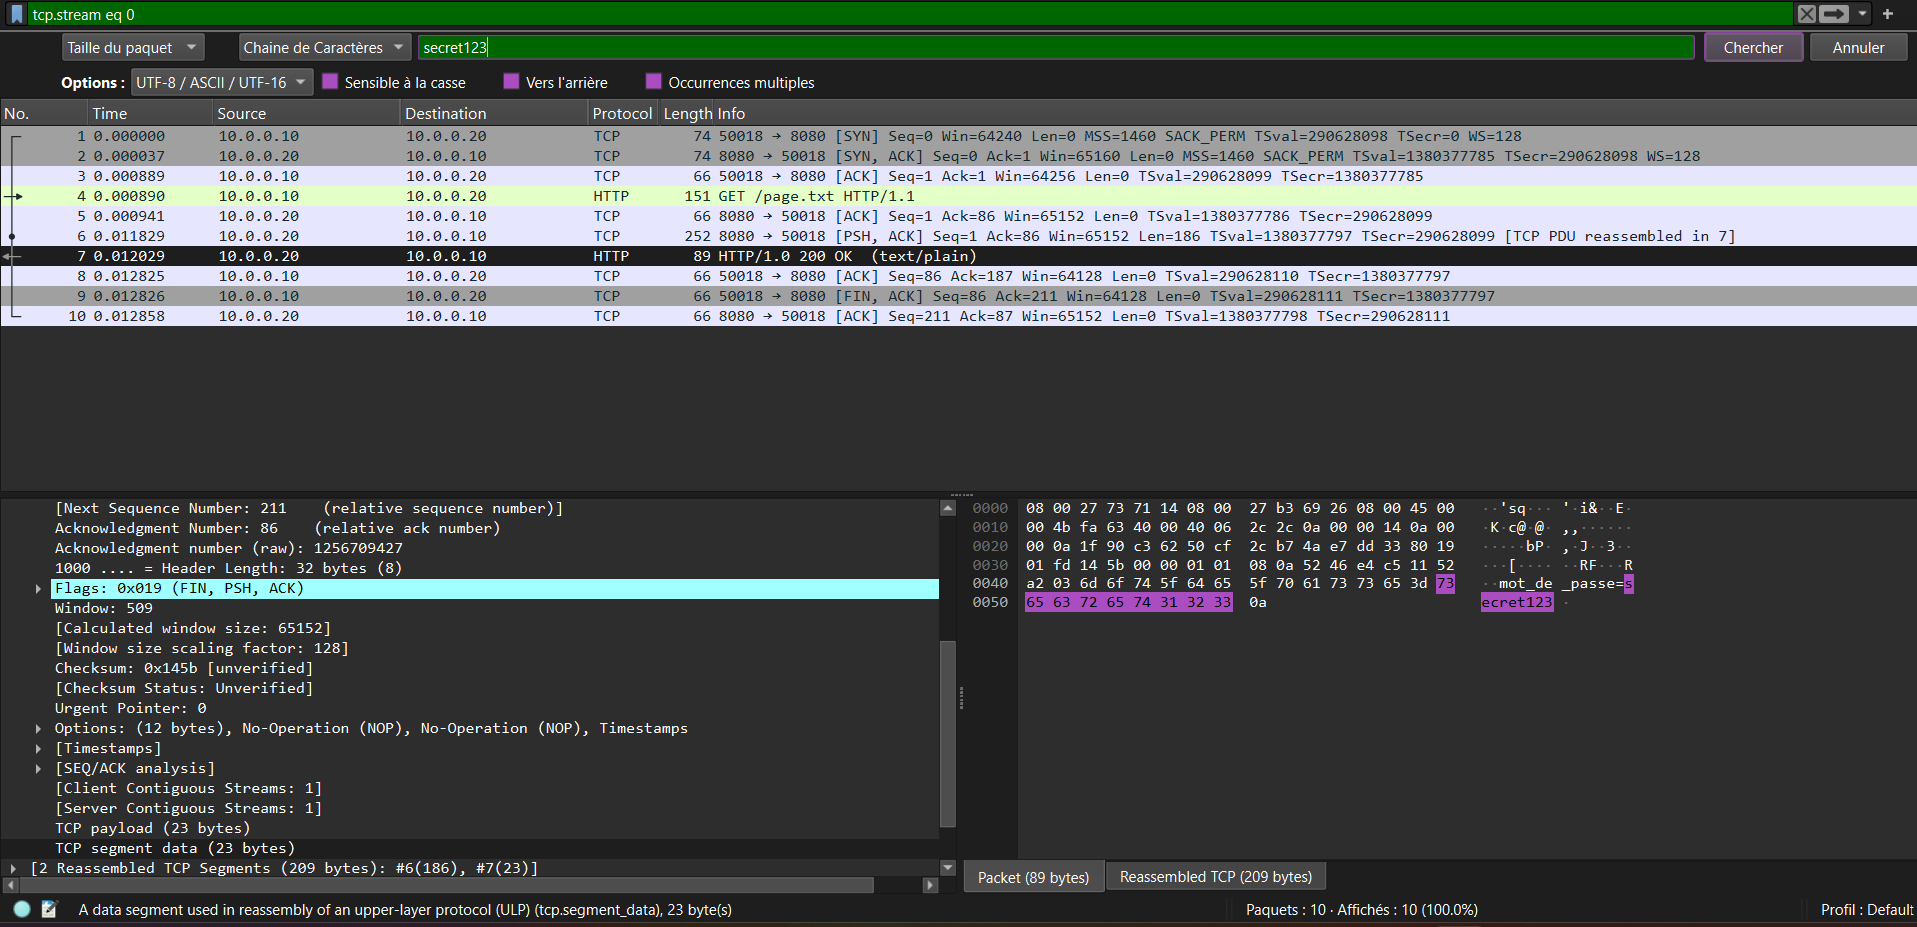
\includegraphics[width=\textwidth]{wireshark_clair_recherche.png}
  \caption{Clair : \texttt{secret123} trouvé}
\end{subfigure}\hfill
\begin{subfigure}{0.48\textwidth}
  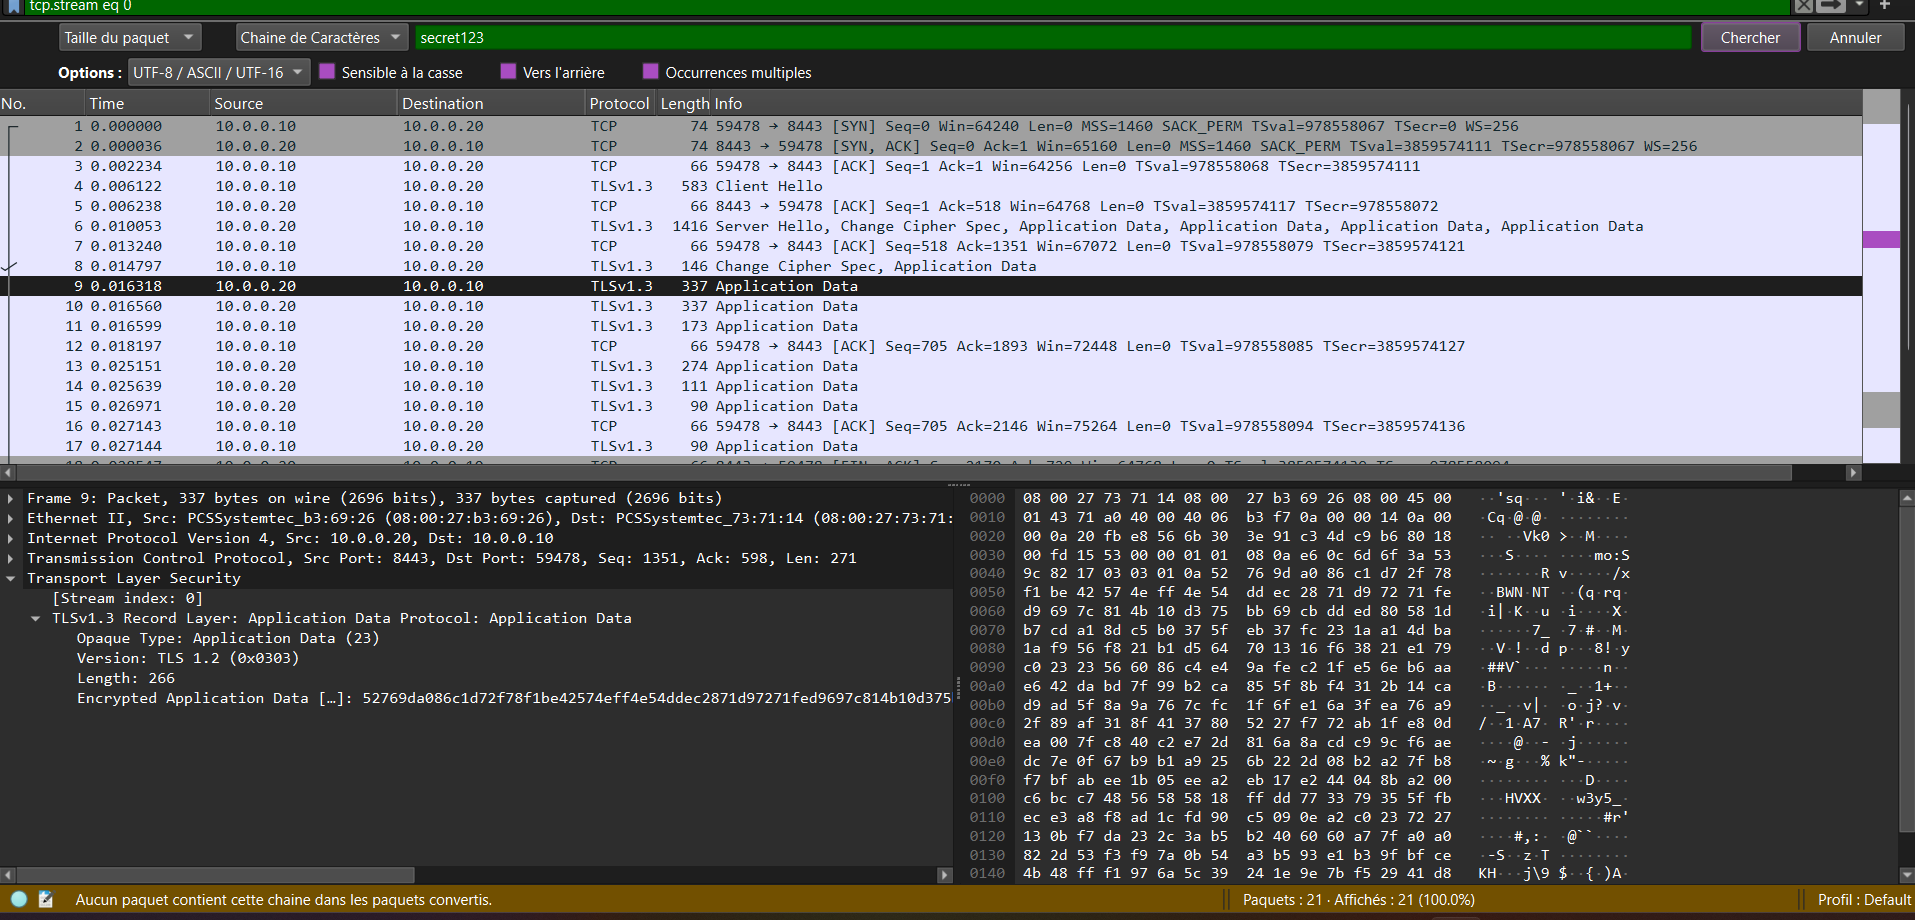
\includegraphics[width=\textwidth]{wireshark_tls_recherche.png}
  \caption{TLS : introuvable}
\end{subfigure}\\[6pt]
\begin{subfigure}{0.48\textwidth}
  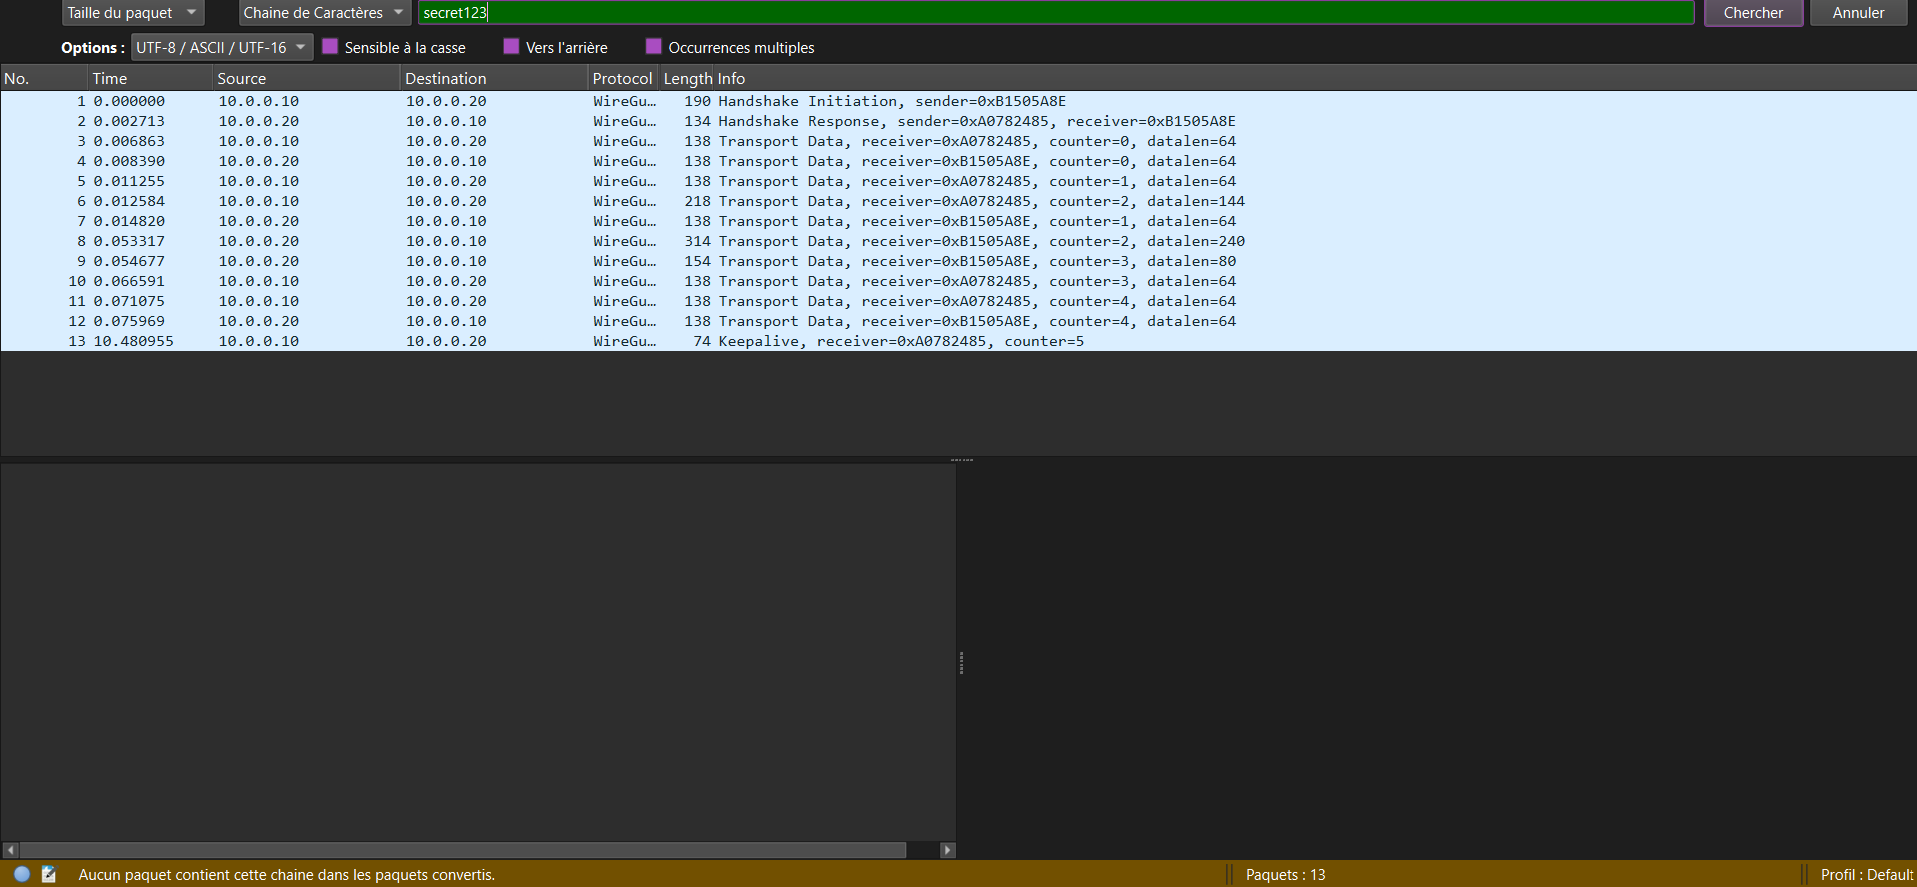
\includegraphics[width=\textwidth]{wireshark_wg_recherche.png}
  \caption{WireGuard : introuvable}
\end{subfigure}\hfill
\begin{subfigure}{0.48\textwidth}
  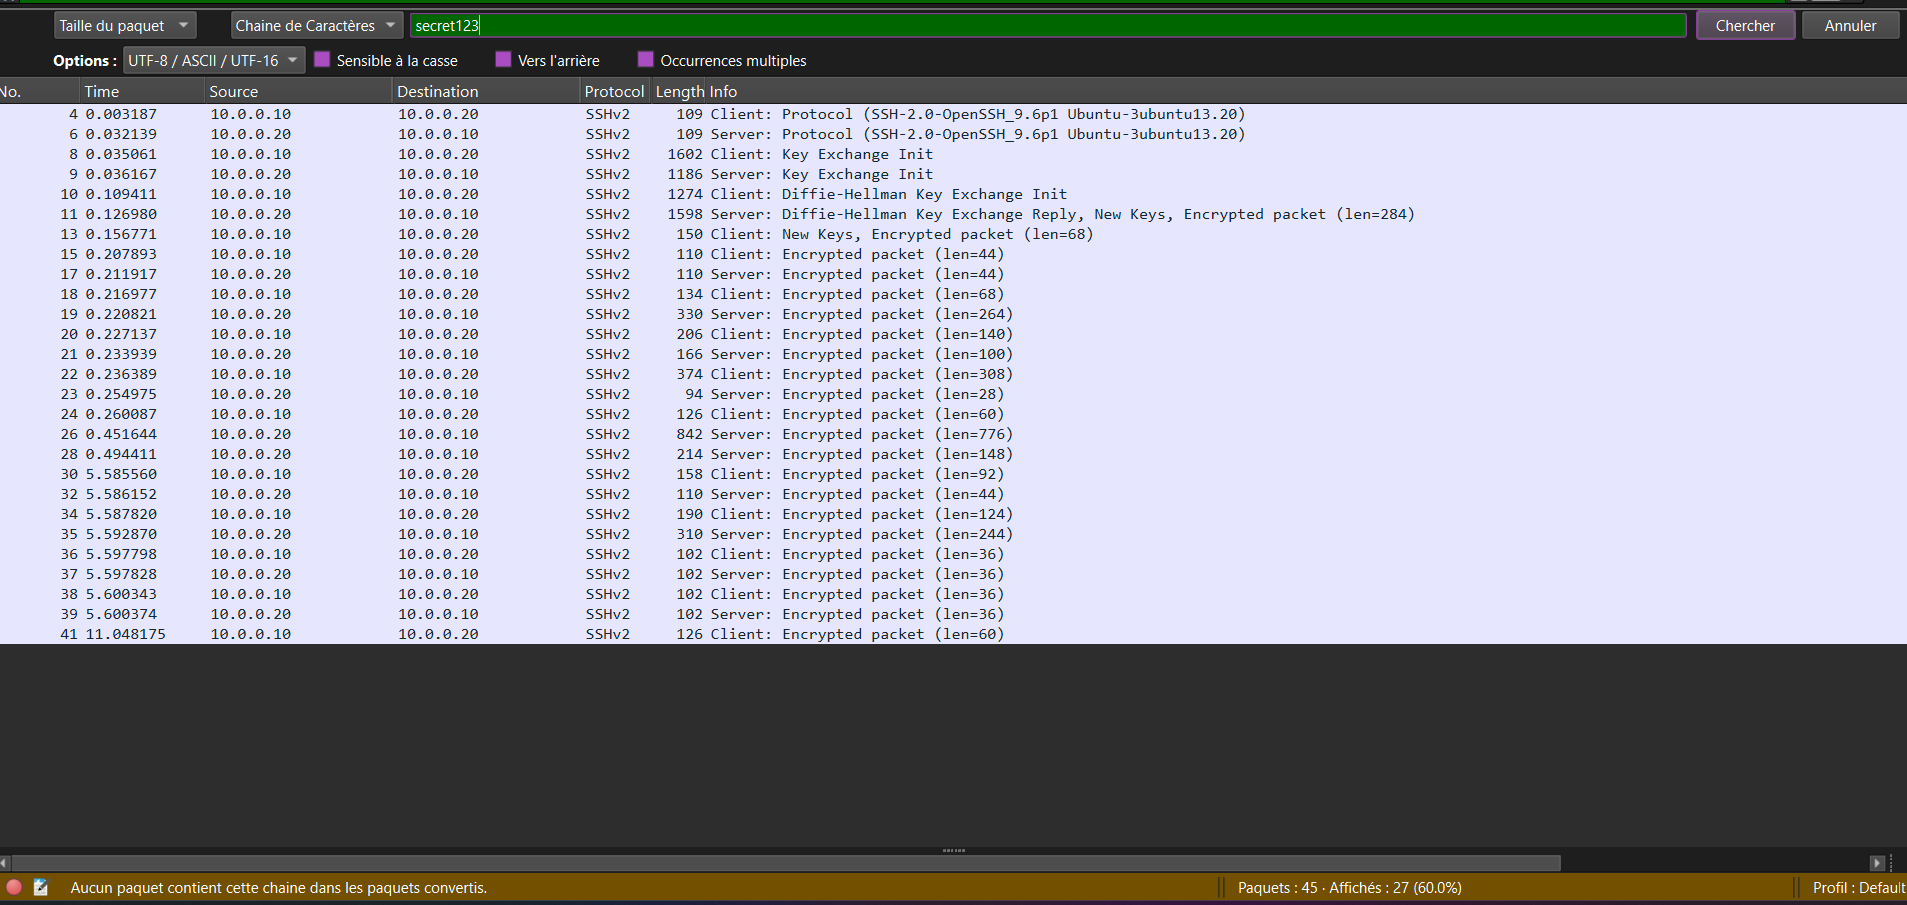
\includegraphics[width=\textwidth]{wireshark_ssh_recherche.png}
  \caption{SSH : introuvable}
\end{subfigure}
\caption{Recherche de la chaîne \texttt{secret123} dans les captures Wireshark.}
\end{figure}

Autres captures : \fic{wireshark\_clair\_flux.png}, \fic{wireshark\_tls\_paquets.png},
\fic{wireshark\_tls\_flux.png}, \fic{wireshark\_wg\_paquets.png}, \fic{wireshark\_wg\_detail.png},
\fic{wireshark\_ssh\_paquets.png}, \fic{wireshark\_ssh\_kex.png}.

\subsection{Analyse}
\begin{itemize}
  \item \textbf{Latence par petite requête} : WireGuard est le moins coûteux des trois protections
        (+4,6~ms), car son tunnel est déjà établi avant la requête : aucune négociation n'a lieu
        à chaque connexion. TLS paie à chaque nouvelle connexion une poignée de main complète
        (13,06~ms, qui explique l'essentiel des 14,69~ms de surcoût mesurés). Le tunnel SSH se
        situe entre les deux : la session est déjà ouverte, mais chaque nouvelle connexion
        applicative relayée (curl) ouvre un nouveau canal à l'intérieur de cette session, ce qui
        ajoute un aller-retour.
  \item \textbf{Débit} : l'ordre s'inverse : clair $>$ TLS $>$ SSH $>$ WireGuard. Une analyse de
        charge processeur (\texttt{top}, \texttt{ps aux}) pendant les transferts WireGuard a montré
        un processeur du Serveur saturé à environ 89~\% (42,7~\% en code noyau, 46,4~\% en
        traitement des interruptions réseau), porté par les threads \texttt{kworker/*-wg-crypt-wg0} :
        le chiffrement de WireGuard, réalisé en espace noyau par logiciel sur un processeur à
        2~vCPU, est le facteur limitant dans cet environnement, et non la configuration ou la
        fragmentation des paquets (vérifiée par un test de MTU sans perte). TLS et SSH, qui
        chiffrent en espace utilisateur dans un seul processus, souffrent moins de cette limite
        dans ce laboratoire.
  \item \textbf{Rôles distincts} : WireGuard protège tout le trafic IP entre deux machines (adapté
        à un VPN site-à-site ou poste-à-site) ; TLS protège une connexion applicative avec
        authentification par certificat (adapté au web, à la messagerie) ; le tunnel SSH par
        redirection de port protège une connexion applicative ponctuelle avec authentification par
        clé (adapté à l'administration ou à un accès temporaire), mais n'est pas un VPN complet.
  \item \textbf{Variabilité} : comme indiqué en méthode, les débits en clair mesurés d'une session
        à l'autre varient de 470 à 1\,228~Mbit/s selon le jour pour une configuration identique.
        Les rapports entre protocoles (−25~\%, −35~\%, −89~\%), mesurés dans une même session,
        sont plus fiables que les valeurs brutes.
\end{itemize}

% ---------------------------------------------------------------------
\section{C4 -- IDS et pare-feu (partie B)}

\subsection{Installation et configuration de Suricata}
Suricata 7.0.3 a été installé sur le Serveur et configuré pour surveiller l'interface
\texttt{enp0s8} (réseau interne) avec \texttt{HOME\_NET: "[10.0.0.0/24]"}. Les règles
\emph{Emerging Threats Open} ont été téléchargées avec \texttt{suricata-update} : 69\,503 règles
chargées, 53\,530 activées, 0 règle en échec. Trois règles locales ont été ajoutées
(\texttt{local.rules}) pour garantir une démonstration fiable, indépendamment des règles génériques :

\begin{lstlisting}
alert icmp any any -> $HOME_NET any (msg:"LAB ICMP echo vers le serveur"; itype:8; sid:1000001; rev:1;)
alert tcp any any -> $HOME_NET any (msg:"LAB Scan de ports SYN"; flags:S; threshold:type both, track by_src, count 15, seconds 5; sid:1000002; rev:1;)
alert tcp any any -> $HOME_NET 22 (msg:"LAB Brute force SSH"; flow:to_server; flags:S; threshold:type both, track by_src, count 10, seconds 10; sid:1000003; rev:1;)
\end{lstlisting}

La configuration a été validée avec \texttt{suricata -T -c /etc/suricata/suricata.yaml}
(\emph{Configuration provided was successfully loaded}) avant chaque démarrage du service.

\subsection{Scénarios de test et détections obtenues}
\begin{itemize}
  \item \textbf{Ping (ICMP)} : 4 paquets envoyés depuis le Client ont produit 4 alertes
        \emph{LAB ICMP echo vers le serveur} journalisées dans \texttt{fast.log}, à la seconde près.
  \item \textbf{Scan de ports} : \texttt{nmap -sS -sV -p 1-2000 10.0.0.20} depuis le Client (un seul
        port ouvert détecté : 22/tcp SSH, en 4 secondes). La règle de seuil \emph{LAB Scan de ports
        SYN} s'est déclenchée, avec le détail complet visible en format \texttt{eve.json}
        (adresses, ports, horodatage, \texttt{"action": "allowed"}).
  \item \textbf{Brute force SSH} : l'outil Hydra 9.5 (bibliothèque SSH fournie par Ubuntu 24.04)
        s'est révélé incapable d'établir une session SSH avec le Serveur, y compris avec le mot de
        passe correct, et ce même après restriction des algorithmes cryptographiques du serveur à
        des valeurs classiques (sans l'échange de clé post-quantique). Le diagnostic en mode debug
        (\texttt{hydra -d}) montre l'échec au niveau de la négociation de session, avant tout envoi
        réel du mot de passe. Ce résultat est documenté comme une limite de l'outil face à une
        configuration SSH moderne (OpenSSH 9.6, clé d'hôte Ed25519), et non comme une résistance du
        service au brute force par mot de passe.

        Pour tout de même démontrer et mesurer la détection d'un brute force, une attaque a été
        simulée par l'ouverture de 15 connexions SSH parallèles en quelques secondes
        (authentification par mot de passe forcée, échec volontaire). Résultat : alerte \emph{LAB
        Brute force SSH} journalisée à chaque vague d'attaque (3 occurrences sur l'ensemble des
        tests, horodatées), avec la source 10.0.0.10 et le port de destination 22 systématiquement
        identifiés.
  \item \textbf{Faux positifs} : un comptage des signatures les plus fréquentes dans
        \texttt{eve.json} sur l'ensemble des jours de test (incluant tout le trafic normal : SSH,
        TLS, WireGuard, iperf3) montre que seules les règles locales se sont déclenchées (4
        occurrences ICMP, 2 occurrences scan) ; aucune règle Emerging Threats Open ne s'est
        déclenchée sur du trafic légitime. Les 53\,530 règles génériques n'ont produit aucun faux
        positif observable dans ce laboratoire restreint -- un résultat positif pour Suricata, à
        nuancer par la faible diversité du trafic testé par rapport à un réseau de production.
\end{itemize}

\begin{figure}[H]
\centering
\begin{subfigure}{0.48\textwidth}
  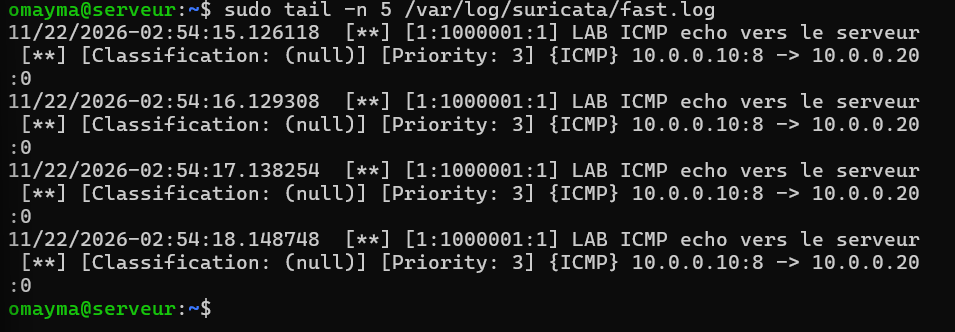
\includegraphics[width=\textwidth]{suricata_alerte_icmp.png}
  \caption{Alertes ICMP}
\end{subfigure}\hfill
\begin{subfigure}{0.48\textwidth}
  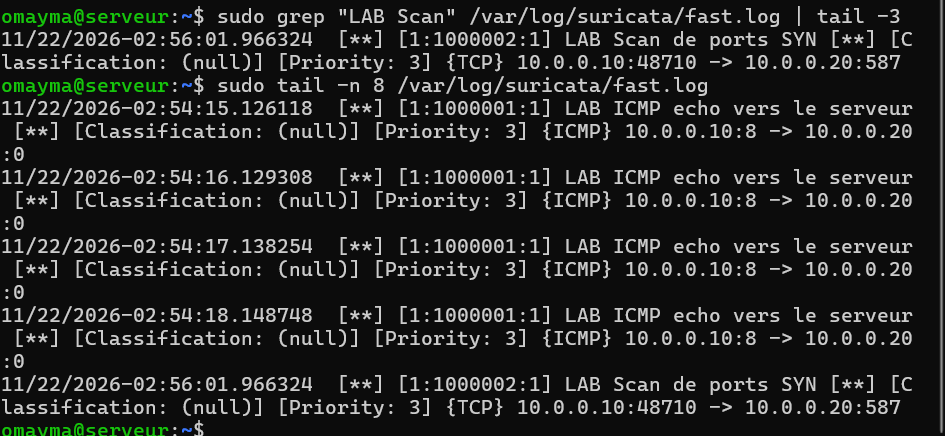
\includegraphics[width=\textwidth]{suricata_alerte_scan.png}
  \caption{Alerte de scan de ports}
\end{subfigure}
\caption{Alertes Suricata journalisées pendant les scénarios de test.}
\end{figure}

Autres captures : \fic{suricata\_config.png}, \fic{suricata\_regles.png},
\fic{suricata\_demarrage.png}, \fic{suricata\_regles\_locales.png}, \fic{suricata\_eve\_json.png},
\fic{suricata\_top\_signatures.png}, \fic{hydra\_echec\_debug.png}, \fic{bruteforce\_simule.png},
\fic{suricata\_alerte\_bruteforce.png}, \fic{nmap\_scan.png}, \fic{suricata\_scan\_alertes.png}.

\subsection{Règles nftables et comparaison avant / après}
Un pare-feu a été configuré sur le Serveur avec une politique par défaut en refus
(\texttt{policy drop}), n'autorisant explicitement que : le trafic de boucle locale, les
connexions déjà établies, ICMP et SSH :

\begin{lstlisting}
table inet filter {
    chain input {
        type filter hook input priority filter; policy drop;
        iif "lo" accept
        ct state established,related accept
        ip protocol icmp accept
        tcp dport 22 accept
    }
}
\end{lstlisting}

Une règle de limitation de débit a ensuite été ajoutée pour borner le nombre de connexions SSH
acceptées par seconde :

\begin{lstlisting}
tcp dport 22 limit rate over 5/second burst 5 packets counter drop
\end{lstlisting}

\begin{table}[H]
\centering
\begin{tabularx}{\textwidth}{l Y Y}
\toprule
\textbf{Indicateur} & \textbf{Avant la règle de limitation} & \textbf{Après} \\
\midrule
Compteur \texttt{drop} de nftables & -- (règle absente) & de 28 à 162 paquets rejetés (134 nouveaux, 30\,728 octets) \\
Connexion SSH légitime isolée & Acceptée & Toujours acceptée (sous le seuil de 5/s) \\
Détection Suricata & Alerte journalisée (\texttt{allowed}) & Alerte journalisée de la même façon \\
\bottomrule
\end{tabularx}
\caption{Effet de la règle de limitation de débit pour une même attaque simulée (15 connexions
SSH parallèles, répétée deux fois).}
\end{table}

\subsection{Analyse : complémentarité IDS / pare-feu}
\begin{table}[H]
\centering
\begin{tabularx}{\textwidth}{l Y Y}
\toprule
 & \textbf{Suricata (IDS)} & \textbf{nftables (pare-feu)} \\
\midrule
Rôle & Observe et journalise & Filtre et bloque \\
Action sur le trafic détecté & \texttt{"action": "allowed"} -- aucune & Rejet effectif (\texttt{drop}), comptabilisé \\
Information produite & Détaillée (signature, adresses, ports, horodatage, JSON exploitable) & Un compteur global (paquets, octets) \\
Limite observée & Ne bloque rien seul ; dépend de la qualité des règles & Règle de seuil simple, pas d'analyse du contenu applicatif \\
\bottomrule
\end{tabularx}
\caption{IDS et pare-feu : deux rôles complémentaires.}
\end{table}

Les deux outils sont complémentaires plutôt que concurrents : l'IDS permet de comprendre une
attaque (qui, quoi, quand), le pare-feu permet de la neutraliser en temps réel. Dans un
déploiement réel, on les associe généralement, voire on relie les alertes de l'IDS à des règles
de blocage automatiques (mode IPS), ce qui dépasse le périmètre de ce laboratoire.

% ---------------------------------------------------------------------
\section{Synthèse comparative et recommandations}

\subsection{Algorithmes et mots de passe (C1, C2)}
\begin{table}[H]
\centering\small
\begin{tabularx}{\textwidth}{l Y Y Y Y}
\toprule
\textbf{Solution} & \textbf{Sécurité} & \textbf{Performance} & \textbf{Complexité} & \textbf{Recommandée pour} \\
\midrule
AES-GCM & Confidentialité + intégrité, rapide, parallélisable & Très élevée (5\,432 Mo/s en AES-128) & Faible (bibliothèques standard) & Chiffrement de données au repos ou en transit, cas général \\
AES-CBC & Confidentialité seule, nécessite un MAC séparé & Élevée mais 3,3$\times$ plus lente que GCM & Risque d'erreur (padding oracle si mal implémenté) & À éviter pour du neuf ; héritage uniquement \\
RSA & Authentification et signature, standard ancien et très répandu & Signature lente (surtout 4096 bits), vérification rapide & Clés et signatures volumineuses & Compatibilité avec des systèmes anciens \\
ECDSA / Ed25519 & Sécurité équivalente à RSA avec des clés bien plus courtes & Signature très rapide (surtout Ed25519) & Faible ; Ed25519 déterministe (pas de piège du nonce) & Nouveaux systèmes, environnements contraints (IoT, mobile) \\
SHA-256 / SHA-3 & Intégrité, résistant aux collisions connues & SHA-2 plus rapide ici & Faible & Empreinte de fichiers, vérification d'intégrité (jamais pour des mots de passe) \\
PBKDF2 / bcrypt / Argon2id & Hachage lent et salé, coût réglable, résiste au brute force hors ligne & Volontairement lent (quelques ms à quelques centaines de ms par hash) & Faible à modérée (paramètres à bien choisir) & Stockage de mots de passe ; Argon2id en premier choix, bcrypt en second \\
\bottomrule
\end{tabularx}
\end{table}

\subsection{Protocoles, IDS et pare-feu (C3, C4)}
\begin{table}[H]
\centering\small
\begin{tabularx}{\textwidth}{l Y Y Y Y}
\toprule
\textbf{Solution} & \textbf{Sécurité} & \textbf{Performance} & \textbf{Complexité} & \textbf{Recommandée pour} \\
\midrule
Clair & Aucune protection & Référence (débit et latence maximaux) & Nulle & Jamais pour un trafic sensible ; référence de mesure uniquement \\
TLS & Confidentialité, intégrité, authentification par certificat & Bon débit, coût concentré à l'ouverture de connexion & Modérée (gestion de certificats et de PKI) & Protection d'une application web ou d'un service exposé publiquement \\
WireGuard & Confidentialité et intégrité de tout le trafic IP, chiffrement moderne imposé & Faible coût par requête, mais débit limité par le CPU en environnement contraint & Faible une fois les clés échangées & VPN site-à-site ou poste-à-site, protection de tout un flux réseau \\
SSH (tunnel) & Confidentialité et authentification par clé, échange post-quantique par défaut & Bon compromis latence / débit & Faible (outil déjà largement répandu en administration) & Accès ponctuel ou administration à distance, pas un VPN complet \\
Suricata + nftables & Détection détaillée (IDS) complétée par un blocage effectif (pare-feu) & Impact mesuré faible sur le trafic normal, charge CPU au chargement des règles & Modérée (règles à écrire et valider) & Surveillance et protection d'un service exposé, en complément des mesures ci-dessus \\
\bottomrule
\end{tabularx}
\end{table}

\subsection{Recommandations par besoin}
\begin{itemize}
  \item \textbf{Chiffrer des données} (fichier, flux applicatif) $\rightarrow$ AES-256-GCM (ou
        AES-128-GCM si la performance prime et que le contexte ne l'exige pas).
  \item \textbf{Signer un message ou authentifier une machine} $\rightarrow$ Ed25519 par défaut pour
        un nouveau système ; RSA-2048 minimum uniquement pour compatibilité avec de l'existant.
  \item \textbf{Stocker des mots de passe} $\rightarrow$ Argon2id avec des paramètres recommandés
        ($m \geq 19$~Mio, $t \geq 2$) ; bcrypt (coût $\geq 10$) si Argon2id n'est pas disponible dans
        l'environnement cible. Jamais de hachage rapide non salé.
  \item \textbf{Protéger un flux applicatif isolé} (site web, API) $\rightarrow$ TLS, pour son
        authentification par certificat et sa large compatibilité.
  \item \textbf{Protéger tout le trafic entre deux sites ou machines} $\rightarrow$ WireGuard, en
        anticipant un besoin de CPU suffisant côté serveur si le débit doit être élevé ; à défaut,
        un tunnel SSH suffit pour un accès ponctuel ou administratif.
  \item \textbf{Détecter et limiter des comportements anormaux} (scan, brute force, trafic excessif)
        $\rightarrow$ associer un IDS (Suricata) pour la détection et la journalisation détaillée à un
        pare-feu (nftables) pour l'action de blocage effective ; aucun des deux seul ne couvre les
        deux besoins.
\end{itemize}

% ---------------------------------------------------------------------
\section{Conclusion, limites et extensions}

Ce projet a permis de configurer, attaquer et mesurer quatre familles de solutions de sécurité,
plutôt que de se contenter de les utiliser telles quelles. Les résultats confirment des principes
connus (AES-GCM plus rapide et plus sûr que CBC, Argon2id préférable à un hachage rapide, le
chiffrement coûte toujours quelque chose) tout en les chiffrant précisément dans un environnement
réel, avec ses contraintes propres (VMs à 2~vCPU, virtualisation, outils d'attaque parfois dépassés
par des configurations modernes).

\textbf{Limites communes}
\begin{itemize}
  \item Mesures réalisées en machines virtuelles, avec un partage de CPU variable d'une session à
        l'autre (écarts de débit observés jusqu'à $\times 2$ pour une configuration identique) ; les
        comparaisons intra-session restent valides, les valeurs absolues moins.
  \item Liste de mots de passe de test courte (1\,000 candidats, 10 comptes) et coûts de craquage
        volontairement réduits (C2), pour rester dans le temps imparti.
  \item Les mesures de C1 et C2 (partie A) et celles de C3 et C4 (partie B) ont été faites dans des
        VMs distinctes (Ubuntu 22.04 pour A, Lubuntu 24.04 pour B) ; elles ne sont donc pas
        comparables entre elles en valeur absolue, ce qui n'est pas nécessaire pour les
        conclusions de ce rapport.
  \item Scénarios d'attaque simulés et contrôlés, sans rapport de volumétrie avec un trafic de
        production réel.
  \item L'outil Hydra, dans sa version disponible, s'est révélé incompatible avec la configuration
        SSH par défaut du Serveur, ce qui a nécessité une attaque simulée en remplacement pour
        démontrer la détection par seuil.
  \item Le débit WireGuard mesuré est spécifique à des VMs à 2~vCPU sans accélération matérielle
        dédiée au chiffrement ; un environnement avec davantage de c\oe urs ou du matériel dédié
        changerait probablement ce résultat.
\end{itemize}

\textbf{Extensions possibles, non traitées faute de temps}
\begin{itemize}
  \item VPN complémentaire (OpenVPN) pour une quatrième comparaison de protocole.
  \item PKI avec gestion de la révocation (CRL), plutôt qu'un certificat auto-signé pour TLS.
  \item Attaque de type \emph{man-in-the-middle} active, en plus de l'observation passive par
        Wireshark.
  \item Comparaison de plusieurs pare-feu (nftables contre iptables, ou contre un pare-feu
        applicatif).
  \item Passage de Suricata en mode IPS (blocage automatique des alertes), pour unifier détection
        et action.
\end{itemize}

% ---------------------------------------------------------------------
\section*{Annexes}
\addcontentsline{toc}{section}{Annexes}
\begin{itemize}
  \item Dépôt du projet : \url{https://github.com/oumayma605/secureai-gateway}
  \item Captures d'écran : \fic{docs/captures/}
  \item Configurations commentées : \fic{config/} (\fic{stunnel.conf}, \fic{wg0\_client.conf},
        \fic{wg0\_serveur.conf}, \fic{nftables\_j6.conf}, \fic{local\_j6.rules},
        \fic{suricata\_j5.yaml})
  \item Scripts : \fic{algorithms/}, \fic{passwords/}, \fic{run\_all\_A.sh}, \fic{vagrant/}
  \item Résultats bruts (CSV, journaux, captures réseau) : \fic{results/}
\end{itemize}

\end{document}
